\documentclass[preprint]{iacrtrans}

\usepackage[utf8]{inputenc}
\usepackage{amssymb, amsmath, amsfonts, amscd}
\usepackage[T1]{fontenc}
\usepackage{graphicx}
\usepackage{url}
\usepackage{xspace}
\usepackage{subcaption}
\usepackage{algorithm2e}
\usepackage{tikz}
\usepackage{cellspace}
\usepackage{multirow}
%\usepackage{parskip}
\usetikzlibrary{patterns}

%\usepackage[noend]{algpseudocode}

\usepackage[pdftex,bookmarks,bookmarksopen,bookmarksdepth=3]{hyperref}
\hypersetup{colorlinks=true,citecolor=red,linkcolor=red,urlcolor=black}

\usepackage{algorithmic}

% knuth-style algos
\newcommand{\slug}{\hbox{\kern1.5pt\vrule width2.5pt height6pt depth1.5pt\kern1.5pt}}
\def\xskip{\hskip 7pt plus 3pt minus 4pt}
\newdimen\algindent
\newif\ifitempar \itempartrue % normally true unless briefly set false
\def\algindentset#1{\setbox0\hbox{{\bf #1.\kern.25em}}\algindent=\wd0\relax}
\def\algbegin #1 #2{\algindentset{#21}\alg #1 #2} % when steps all have 1 digit
\def\aalgbegin #1 #2{\algindentset{#211}\alg #1 #2} % when 10 or more steps
\def\aaalgbegin #1 #2{\algindentset{#2111}\alg #1 #2} % when 10 or more steps
\def\alg#1(#2). {\medbreak % Usage: \algbegin Algorithm A (algname). This...
  \noindent{\bf#1}({\it#2\/}).\xskip\ignorespaces}
\def\algstep#1.{\ifitempar\smallskip\noindent\else\itempartrue
  \hskip-\parindent\fi
  \hbox to\algindent{\bf\hfil #1.\kern.25em}%
  \hangindent=\algindent\hangafter=1\ignorespaces}
% end of borrowed macros

\newcommand{\todo}[1]{\textcolor{red}{TODO:[#1]}}

\title{Predicting the PCG PSeudo-Random Number Generator In Practice} 

\author{Charles Bouillaguet\inst{1} \and Julia Sauvage\inst{2} \and Florette Martinez\inst{3}}


\institute{% 
University of Lille, France \\ 
\email{charles.bouillaguet@univ-lille.fr}
\and 
Sorbonne University \\
\email{julia.sauvage@etu.upmc.fr}
\and 
LIP6, CNRS, SU ? \\
\email{florette.martinez@lip6.fr}

}

\begin{document}
\maketitle

\keywords{keywords}

\begin{abstract}
  blablabla
\end{abstract}

\section{Introduction} %ce qu'on avait écrit pour le projet, peut-être pas incroyable...

\todo{Ca, c'est du blabla...}

Pseudo-random generators (PRG) are well-studied primitives in symmetric
cryptography. A PRG is an efficient deterministic algorithm that stretch a small
random seed into a longer pseudo-random stream. To achieve cryptographic-grade
pseudo-randomness, a PRG must ensure that the pseudo-random stream is
computationally indistinguishable from a ``truly'' random sequence of bits by
efficient adversaries. Alternatively, it is possible to define pseudo-randomness
by asking that no efficient algorithm is capable of predicting the next
pseudo-random bit with non-negligible accuracy. The two definitions are in fact
equivalent.

\todo{mentioner stream ciphers}

Not all pseudo-random generators are of cryptographic strength. In some
applications, it is not necessarily necessary: to be used in Monte-Carlo
simulations or generate random choices in games, a relaxed, non-cryptographic
notion of pseudo-randomness may be sufficient. This allows for faster
algorithms. For instance, the \texttt{Math.Random} function in Google's V8
open-source JavaScript engine uses the \textsf{XorShift128} generator, which is
a Linear Feedback Shift Register tailored for high software speed. On 64-bit
processors, it produces 64 pseudo-random bits with 3 shifts and 4 XORs
instructions. The \textsf{python} standard library's \texttt{random} module uses
the Mersenne Twister. The \textsf{C} library that comes along \texttt{gcc} (the
\texttt{glibc}) uses a (poor) truncated linear congruential generator by default
to implement the \texttt{rand} function.

In the realm of non-cryptographic random generators, a PRG is deemed ``good
enough'' it is passes \emph{some} efficient statistical tests --- whereas the
cryptographic notion of pseudo-randomness asks that it passes \emph{any}
efficient test. There are \textit{de facto} statistical test suites (\todo{les
  mentionner}). The goal of designers then consists in designing the fastest
possible generator that passes the day's favorite test suite.

\todo{Mentionner Ferrenberg 92}

The scientific computing community also realized that the need for fast
\emph{parallel} random number generation could be satisfied by the use of block
ciphers in counter mode~\cite{Salmon11}. The need for speed then leads to the
use of weakened cryptographic primitives.

In most cases, it is easy to see that a non-cryptographic PRG does not meet the
cryptographic notion of pseudo-randomness, and there are few exceptions. In this
paper, we study the \textsf{PCG} family of non-cryptographic pseudo-random
generators~\cite{melissapaper,melissaweb}.

\textsf{PCG} stands for ``Permuted Congruential Generator'': it essentially
consists in applying a non-linear filtering function on top of a (fairly weak)
linear congruential generator (in a way reminiscent to the venerable filtered
LFSRs). The resulting combination is fast and passes current test suites. Its
designer claimed that distinguishing the pseudo-random stream produced would be
``challenging''. The \textsf{PCG} family contains many members, but we focus on
its strongest member, named either \textsf{PCG64} or \textsf{PCG-XSL-RR}. It has
a 128-bit internal state and produces 64 bits when clocked. It is the default
pseudo-random number generator in the popular \textsf{NumPy} scientific
computing package for \textsf{Python}.

The internal state of the \textsf{PCG64} generator is made of a 128-bit
``state'' and a 128-bit ``increment'', whose intended use is to provide several
pseudo-random streams with the same seed (just as the initialization vectors do
in stream ciphers). A default increment is provided in case the end-user just
want one pseudo-random stream with a single 128-bit seed.

\paragraph{Contribution.} We describe an algorithm that reconstructs the full
internal state of the strongest member of the \textsf{PCG} family. This allows
to predict the pseudo-random stream deterministically and clock the generator
backwards. The original seeds can also easily be reconstructed. The algorithm is
practical and we have executed it in practice. It follows that predicting the
output of the \textsf{PCG} should not be considered challenging anymore.

Our algorithm reconstruct the internal state using the ``guess-and-determine''
technique: some bits of the internal state are guessed ; assuming the guesses
are correct, some other information is computed ; a consistency check discards
bad guesses early on ; then candidate internal states are computed and fully
tested. The problem actually come in two distinct flavors.

When the increment is known (for instance when it is the default value), a
simplified prediction algorithm recovers the internal state from 192 bits of
pseudo-random stream. The process runs in 20 CPU minutes (on a single core of a
server processor). It guesses 36 bits of the internal state, then solves an
instance of the \textsc{Closest Vector Problem} (CVP) in a 3-dimensional
euclidean lattice. This requires about 50 arithmetic operations in total and
reveals the entire internal state if the guesses are correct.

When the increment is unknown, things are a bit more complicated. This is the
default situation in \textsf{NumPy}, where both the state and the increment are
initialized using an external source of entropy. In this case, our prediction
algorithm requires 3072 bits of pseudo-random stream ; it guesses between 51 and
55 bits, then for each guess it solves and instance of CVP in dimension 4 (using
about 75 arithmetic operations). This recovers 64 more bits of information about
the difference between two successive states, and this is enough to filter the
bad guesses. This information can then be used in a subsequent and comparably
inexpensive phase to recover the entire internal state. On average, the whole
process requires a bit less than 20 000 CPU hours to complete.

We implemented the algorithms in \textsf{C}, then asked the designer of the PCG
family to send us ``challenge'' pseudo-random streams ; we ran our code and
emailed back the seeds used to generate the challenge streams the next day.

\paragraph{Related Work.} \todo{Mentionner Knuth et les LCG + Frieze + Boyar + Stern...}

\todo{mentionner Vigna ?}

% The combination between being highly commended (it achieved 5th place out of 29
% in a recent performance test survey\cite{survey}) and a well presented
% website\cite{melissaweb} giving an feeling of professionalism can lead to the
% impression that PCG is a sufficiently secure family of generators.

% Some attacks against PCG have been carried out by Sebastiano
% Vigna\cite{vignaweb}, but this didn't yield any significant results, given that
% he only tried to break an incomplete version in a fairly straightforward way. He
% worked on a very specific version of PCG. He considers the result without
% modulo, which is a big simplification. Moreover, he didn't study the 128 bits
% long generator, but only the 64 bits long\cite{vignacode}.


\section{The PCG Pseudo-Random Number Generator Family}

\todo{cette section doit décrire précisément PCG.}

\begin{quote}
  In addition, one of the generators, PCG-XSL-RR(described in Section 6.3.3), is
  explicitly designed to make any attempt at state reconstruction especially
  difficult, using xor folding tominimize the amount of information about
  internal state that leaks out.
\end{quote}

\begin{quote}
  Although these properties make it extremely challenging for an agent observing
  theexternal behavior of a program to guess the state of its random number
  generator,
\end{quote}

% import numpy
% print(numpy.random.default_rng())
% ---> Generator(PCG64)

\subsection{LCG algorithm}

The PCG algorithm we studied is based on the Linear Congruential Generators algorithm. The LCG algorithm is simply based on a congruential multiplication. This type of generator is based on four values: an internal state $S_{i}$, a multiplier $A$, an increment $C$ and the size $M$. Generally, to initialize a generator of a given size, a seed value is provided as the first internal state, and a default multiplier and increment are used. We will study the case where $M$ and $A$ are known and where $M$ is a power of 2.\\

Calling the generator results in calculating the next internal state $S_{i+1} = A \times S_i + C \mod{M}$ and outputting $S_{i+1}$ as data.

This type of generator is trivially predictable because, the internal state is given to us at each output, and in the event that $C$ is unknown, we can still deduce it with two consecutive outputs: $C = S_{i+1} - A \times S_i$.\\

A better variant of the standard LCG is the Truncated LCG, where the output consists only of the higher bits of the internal state $S_i$. This way the entire internal state isn't accessible. Returning the lower bits is not interesting because as we can understand easily and will prove later, lower bits of a state only depend on the lower bits of the previous state.

\subsection{PCG algorithm}

The PCG algorithm we studied is based on the LCG algorithm. To start, here are a few definitions:
\begin{itemize}
    \item let $k$ be the size of our generator, in this case $k = 128$ bits;
    \item let $M$ be the modulus with $M = 2^k$;
    \item let $S_i$ be the internal state at the $i$-th iteration and $S$ be the list of $S_i$;
    \item let $X_i$ be the output at the $i$-th iteration of the generator and $X$ be the list of $X_i$;
    \item let $lowS_i$ be the $k/2$ least significant bits of $S_i$;
    \item let $upS_i$ be the $k/2$ most significant bits of $S_i$;
    \item let $rot_i$ be the 6 most significant bits of $S_i$;
    \item let $nbiter$ be the number of consecutive outputs for prediction purposes.
\end{itemize}

The internal state can be redefined as:
\begin{equation}
    S_i = 2^{k/2} \times upS_i + lowS_i 
\end{equation}

The 6 most significant bits, $rot_i$, of the internal state are used as a value to determine the rotation in the PCG algorithm. Let \texttt{rotate} be the function that performs said rotation (Figure \ref{pcg128out}).\\
The rotation is a simple exchange of bits, where a $k/2$ bit value is split into 2 parts: one of $rot_i$ bits and the other in $(k/2) - rot_i$ bits. The two parts are then swapped, and the new value is returned. 

This generator is initialised with a given $k$ bit internal state $S_0$ (of size 128 bits in the case of PCG128), and optionally with an $k$ bit increment $C$. If no increment is given, the algorithm will use a known default increment. For each output of the generator, the algorithm will perform the following calculations" (Figure \ref{pcg128out}):\\
\begin{align}
    X_{i} &= \mathtt{rotate}(upS_i\ \mathtt{XOR}\ lowS_i)\\
    S_{i+1} &= A \times S_{i} + C \mod{2^k}
\end{align}
In the case of PCG128, $A$ is a default increment of size 125 bits prime with $2^k$.

\begin{figure}[h!]
    \centering
    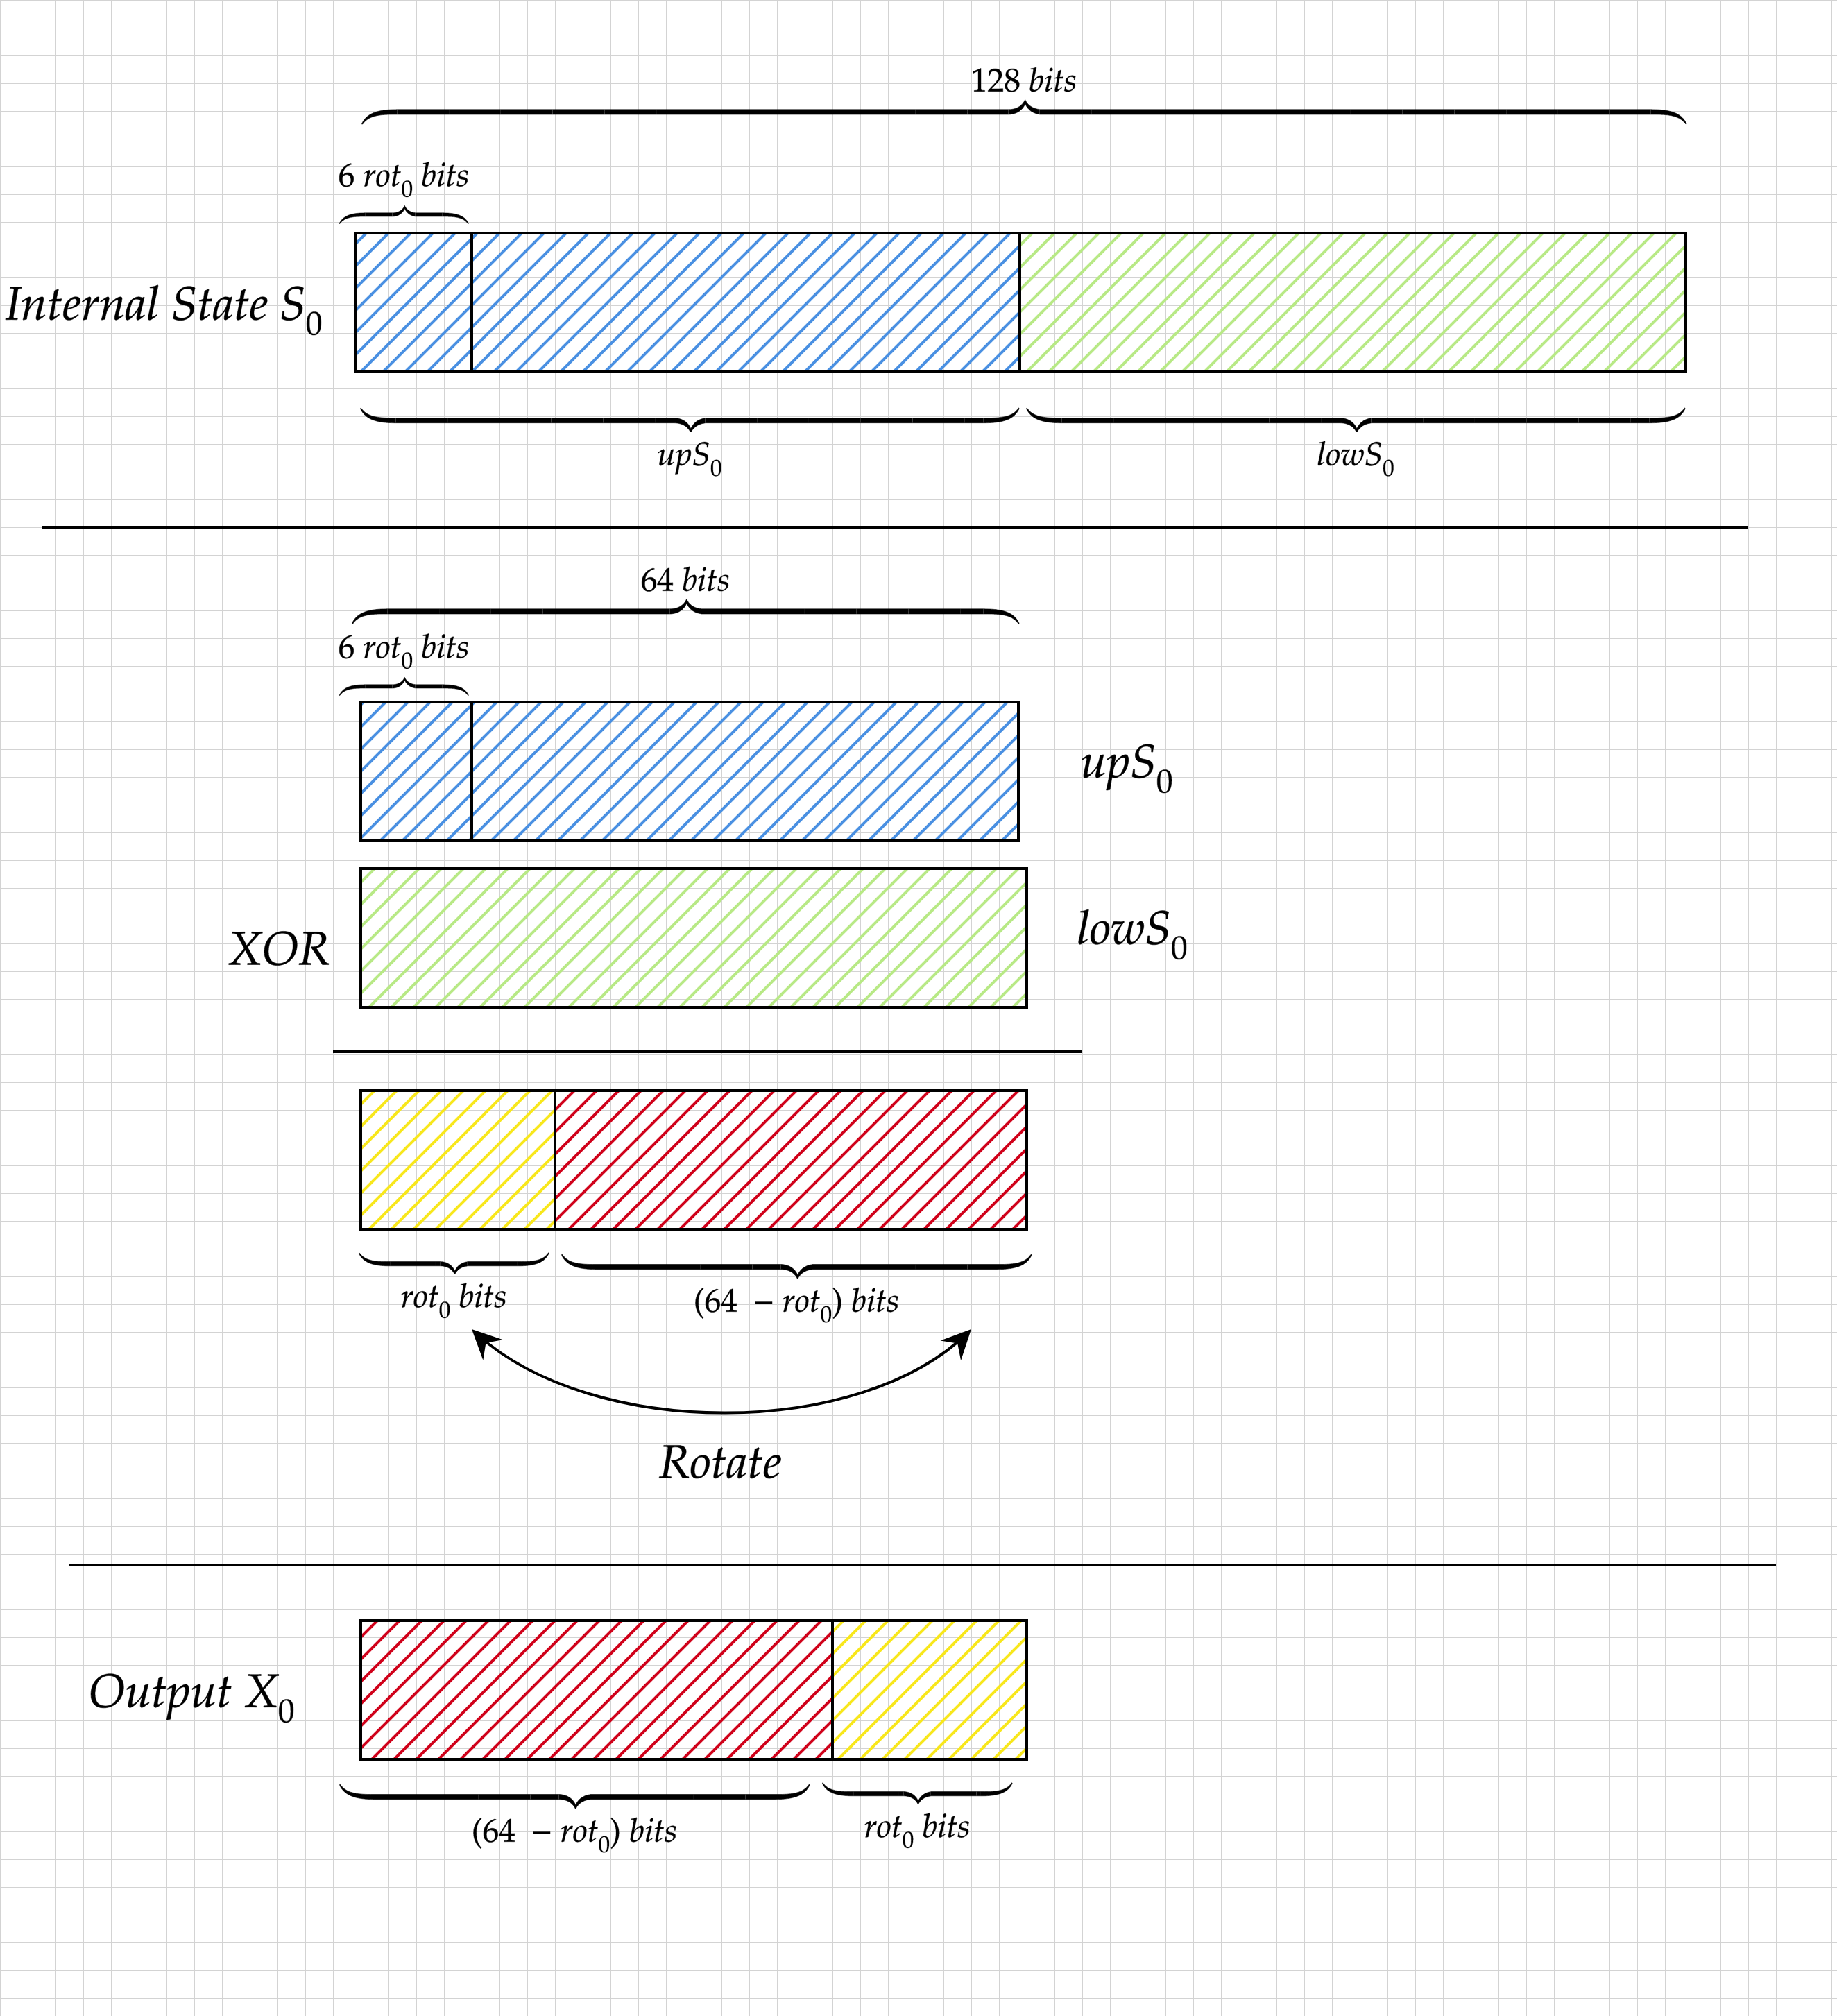
\includegraphics[width=0.75\linewidth]{pictures/PCG128.png}
    \caption{PCG128 : Output process}
    \label{pcg128out}
\end{figure}



Given the nature of the generator, the following values are known at every step:
\begin{itemize}
    \item the size of the generator $k$;
    \item the list of outputs $X$;
    \item the multiplier $A$;
    \item and eventually $C$, if the default increment was used. 
\end{itemize}

To break this generator, we had to differentiate between cases when the default $C$ was used or not. It was also interesting to note what was the minimum number of $X_i$ needed to reliably attack it.





\section{Predicting Truncated Linear Congruential Generators}

\todo{Comme on utilise à plusieurs reprise l'idée de se ramener à un LCG
  tronqué, autant décrire la technique à base de réseaux un bon coup.}

The algorithm of Frieze \textit{et al}\cite{Frieze} solves the case where $M$
and $A$ are known, $M$ being a power of two and, possibly with a significant
portion of the internal state unknown. The known part is the upper bits of the
state. This algorithm is coherent with our problem, this being the reason why we
focused on this one in particular. However, this algorithm won't work for some
particular multipliers. But this problem doesn't concern us, because the default
multiplier of \texttt{PCG128} is not one of them.

The first article we found was written by Joan Boyar\cite{Boyar1989}. The
subject of her study was a special case of truncated LCG, with $A$, $C$ and $M$
unknown and has access to a very large part of the internal state. This made it
so that we couldn't use her findings, because guessing a large part of the
internal state wouldn't be cost-effective. However, her study included a very
broad state of the art, explaining the specifics of many algorithms, as well as
describing in which circumstances they should be used.



\section{C connu}

\subsection{Réduction}
Pour deviner l'état interne du générateur, une méthode consiste à procéder par brute-force. On devine les 64 bits supérieurs de $S_0$, on en déduit la rotation $r_0$ utilisée, on peut retrouver  les 64 bits inférieurs:

\begin{equation}
   S_0[0:64] = S_0[64:128] \texttt{ XOR } \texttt{ROT}(X_0 , 64 - r_0) \\
\end{equation}

Cette méthode demanderait de l'ordre de $2^{64}$ calculs, ce qui n'est pas acceptable. Nous pouvons cependant utiliser cette équation pour déduire des informations sur l'état interne de S. En effet,en devinant par brute-force les 6 bits du haut de S, et ses $\ell$ bits du bas, on récupère :\\% schéma "relevant bits of the outputs"

On réduit $S$ à une série géométrique plus simple. Notons $S'$ l'état interne auquel on retire sa composante en $C$, et en $S_0[0:\ell]$ (note de bas de page : le fait de retirer $S_0[0:\ell]$ n'est pas nécéssaire, mais nous permet de limiter la taille des instances utilisées à 64 bits, très utile pour la programmation en C). Nous utiliserons le réseau engendré par les $S'[\ell : 64 + \ell]$, de matrice génératrice :\\
\begin{equation}
M =
\begin{pmatrix} 
1 & \alpha & \alpha ^2 & \dots & \alpha ^{nbiter - 1}\\
0 & M & 0 & \dots & 0\\
0 & 0 & M & \dots & 0\\
\vdots & & & \ddots & \vdots\\
0 & 0 & \dots & 0 & M
\end{pmatrix}
\end{equation}

\subsection{Algorithme}
On calcule préalablement les matrices $G$ et $G^{-1}$, avec $G$ la matrice génératrice réduite du réseau blablabla par l'algorithme LLL.
Pour tous les $r_i$ et les $S_0[0 : \ell]$ possibles:\\
\begin{enumerate}
\item On récupère le $T$ correspondant à nos suppositions. On calcule $T'$. ($T'_i = (S_i[64 - 6 : 64 + \ell] - (a^i*S_0[0 : \ell] + C * \sum_{j = 0}^i a^j)[64 - 6 : 64 + \ell]) * 2^{64 - 6 - \ell}$)
%schema T et T'
Notons cependant que les composantes en $C$ et $S[0:l]$ sont calculées en dehors de la boucle et stockées dans un tableau pour des raisons de performance. Ceci est fait de même dans tous les algorithmes suivants.

\item We get the correspondant $S'[\ell : 64 + \ell]$ by using the babai rounding technique on $T'$ using $G$ and $G^{-1}$.

\item We test our solution by computing $S_0$ and testing if the following internals states are coherent with the PCG outputs. If the results are coherents, we return $S_0$.

\end{enumerate}


\section{babairounding}

We call \(S't\) the truncated vector : \(S'[\ell,64+\ell]\).

We consider the case were we successfully guessed the 6 upper bits of each \(S_i\) and the \(\ell\) lower bits of \(S_0\). Then we know the \(6+\ell\) upper bits of \(S't\).

(à détailer ?)	

We had define \(S'\) such that \(S'\) is in the lattice \(L(A,2^{128},n)\) and its \(\ell \) lower bits are 0. Then \(S't\) is in \(L(1,2^{64},n)\).

If we consider the vector \(T'\) computed in step (numerodelastepenquestion), we notice it is close to \(S't\) in the sense of they have exactly the same \(6+\ell\) upper bits. So we want to recover \(S't\) by solving an approach \(CVP(L(A,2^{64},n),T')\).

Now we need to prove that the \(pwet\) obtained with the Babai rounding is indeed \(S't\).

We denote \(r = rounding(YG^{-1}) \).

\begin{align*}
\lVert S't - pwet \rVert &= \lVert S't - rG \rVert \\
&= \lVert S't - (r-YG^{-1} + YG^{-1})G \rVert\\
&= \lVert S't - Y + (r-YG^{-1})G \rVert\\
&\leqslant \lVert S't - Y \rVert + \lVert(r-YG^{-1})\rVert \times \lVert G\rVert\\	
\end{align*}

By definition, \(r\) is the closest integer vector to \(YG^{-1}\). But as \(S't\) is an element of the lattice, \(S'tG^{-1}\) is an integer vector. Thus \(r-YG^{-1}\) is smaller than \(S'tG^{-1}-YG^{-1}\).

Hence :
\begin{align*}
\lVert S't - pwet \rVert &\leqslant \lVert S't - Y \rVert + \lVert(r-YG^{-1})\rVert \times \lVert G\rVert\\	
&\leqslant \lVert S't - Y \rVert + \lVert(S'tG^{-1}-YG^{-1})\rVert \times \lVert G\rVert\\	
&\leqslant \lVert S't - Y \rVert + \lVert(S't-Y)\rVert \times \lVert G^{-1} \rVert  \times \lVert G\rVert\\
& 	\leqslant \lVert S't - Y \rVert \times (1 +\lVert G^{-1} \rVert  \times \lVert G\rVert )\\
\end{align*}

But, by construction of \(Y\), we have that \(\lVert S't - Y \rVert \leqslant \sqrt{n2^{2(58-l)}} \). So

\[ \lVert S't - pwet \rVert \leqslant \sqrt{n2^{2(58-l)}}\times (1 +\lVert G^{-1} \rVert  \times \lVert G\rVert )\]\\




Now all we need to do is find sets of parameters \((n,l)\) such that the following inequality is satisfied: 
\[\sqrt{n2^{2(58-\ell)}} \times (1 +\lVert G^{-1} \rVert  \times \lVert G\rVert) \leqslant \lVert SVP(L(A,2^{64},n))\rVert \].

We notice that only the left term of the inequality depends on \(\ell\).

Hence, some sets of parameters that satisfies this inequality are :
\begin{itemize}
	\item \(n = 3\) and \(\ell \geqslant 19\)
	\item \(n = 4\) and \(\ell \geqslant 13\)
	\item \(n = 5\) and \(\ell \geqslant 11\)
	\item \(n = 6\) and \(\ell \geqslant 8\)
\end{itemize}

[insert here] attack predicting algo description.

\begin{theorem}
  The algorithm described above works with probability.... in time ...
\end{theorem}

\section{Predicting PCG with Unknown Increment}
We can't use the same algorithm for the general case. We don't known $C$, so we used an other geometric reduction.
$(\Delta S_{i+1}S_i)_i$ est un suite géométrique de raison $a$.

On calcule préalablement les matrices $G$ et $G^{-1}$.

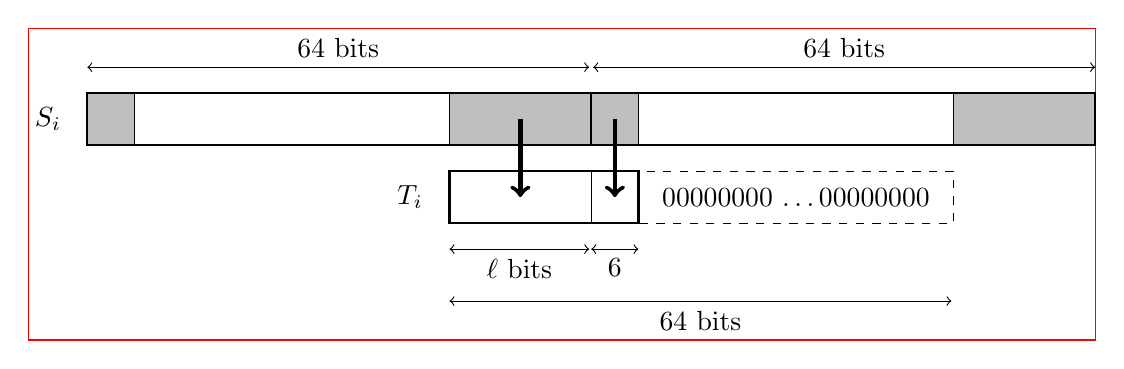
\begin{tikzpicture}[yscale=0.66]
  \draw[red, use as bounding box] (-0.75, -3.75) rectangle (12.8, 2.25);
  
  % S_i
  \begin{scope}
    % remplissage
    \fill[fill=lightgray] (4.6, 0) rectangle +(2.4, 1);
    \fill[fill=lightgray] (0, 0) rectangle +(0.6, 1);
    \fill[fill=lightgray] (11, 0) rectangle +(1.8, 1);
    
    % bordures
    \draw[thick]  (0, 0) rectangle (12.8, 1);
    \draw  (0.6, 0) rectangle +(0, 1);
    \draw[thick]  (6.4, 0) rectangle +(0, 1);
    \draw  (7.0, 0) rectangle +(0, 1);
    \draw  (4.6, 0) rectangle +(0, 1);
    \draw  (11, 0) rectangle +(0, 1);
    
    % déco autour
    \node at (-0.5, 0.5) {$S_i$};
    \draw[<->] (0, 1.5) -- node[above] {64 bits} +(6.375, 0);
    \draw[<->] (6.425, 1.5) -- node[above] {64 bits} +(6.375, 0);
  \end{scope}

  % T_i
  \begin{scope}[xshift=4.6cm, yshift=-1.5cm]    
    \draw[dashed]  (0, 0) rectangle +(6.4, 1);
    \draw[thick]  (0, 0) rectangle +(2.4, 1);
    \draw[]  (1.8, 0) rectangle +(0, 1);
    \path (2.4, 0) rectangle node {00000000 \dots 00000000} (6.4, 1);

    % déco
    \node at (-0.5, 0.5) {$T_i$};
    \draw[<->] (0, -0.5) -- node[below] {$\ell$ bits} +(1.775, 0);
    \draw[<->] (1.8, -0.5) -- node[below] {6} +(0.6, 0);
    \draw[<->] (0, -1.5) -- node[below] {64 bits} +(6.375, 0);
  \end{scope}

  % flèches S_i --> T_i
  \draw[ultra thick,->] (5.5, 0.5) -- +(0, -1.5);
  \draw[ultra thick,->] (6.7, 0.5) -- +(0, -1.5);
  
\end{tikzpicture}

\subsection{Part 1 : Premier filtre}
Pour tous les $r_i$, les $S_0[0 : \ell]$ et les $C[0 : \ell]$ possibles:
\begin{enumerate}
  \item On récupère le $T$  correspondant à nos suppositions. On calcule $\Delta T$ :
  \begin{equation}
    \Delta T_i = (S_{i+1}[58 : 64 + \ell] - S_i[58 : 64 + \ell] - (S_0[0:\ell] * (a^{i+1} - a^i) + C[0:\ell] * a^i )[58 : 64 + \ell]) * 2^{64 - l - 6}
  \end{equation}
  On peut donc aussi définir $\Delta T_i = T'_{i+1} - T'_{i}$ avec $T'$ dont on aurait soustrait la composante en $C[0:\ell]$ et non en $C$.

  \item We get the correspondant $\Delta S_0S_1[0 : 64 + \ell]$ by using the babai rounding technique on $\Delta T$ using $G$ and $G^{-1}$.

  \item On teste s'il existe pour l'itération suivante au moins une rotation $r_n$ cohérente avec le $\Delta T$ trouvé. Pratiquement, pour chacune des 64 $r_n$ possibles, on teste si :
  \begin{align}
     \Delta S_0S_n[0:l] &= S_0[64:64 + l] XOR \mathtt{ROT(X_n , 64 - r_n)[0:l]}\\
     r_n &= S_0[58:64] XOR \mathtt{ROT(X_n , 64 - r_n)[58:64]}
  \end{align}
  Si un de ces égalité n'est pas vérifiée, la solution n'est pas retenue, on passe à la prochaine itération.

  \item On répète la dernière opération encore 3 fois.
\end{enumerate}
Cette première partie de l'algorithme comporte l'énorme majorité du temps de calcul, c'est donc sur elle que doit se porter la recherche de performance.


\subsection{Part 2 : Récupération de la différence complète et deuxième filtre}
On calcule préalalement H matrice génératrice du réseau Lblablabla2 réduite par la méthode LLL.
On a récupéré de la Part 1 une série de $S_0[0 : \ell]$, $r_i$ (i = 0, ..., n) et $C[0 : \ell]$ parmi lequels se trouve notre solution.
\begin{enumerate}
  \item recupérer toutes les $r_i$ possibles, pour $n \leq i \leq m$  par la même méthode que l'étape 3 de la Part 1, répétée $m-n$ fois. On garde en mémoire toutes les rotations possiles.
  \item Pour chacune des $r$ possibles
  \begin{enumerate}
    \item We cumpute $\Delta r$ avec le même méthode que pour $\Delta T$ : 
    \begin{equation}
      \Delta r_i = (S_{i+1}[122 : 128] - S_i[122:128] - (S_0[0:\ell] * (a^{i+1} - a^i) + C[0:\ell] * a^i )[122:128]) * 2^{64 - l - 6}
    \end{equation}
    \item We get the correspondant $\Delta S'_0S'_1$ ($S'$ dont on aurait retiré que ) computing $\texttt{CVP}(r * 2^{128 - \ell}, Lblablabla2)$. We use the fpylll python library CVP function. On stocke le $DS_0S_1$ correspondant.
  \end{enumerate}
\end{enumerate}

\begin{theorem}
  The algorithm described above works with probability.... in time ...
\end{theorem}

\section{Implementation of the Predictor and Practical Results}

\section{Conclusion}

\bibliographystyle{alpha}
\bibliography{biblio}

%\appendix

\end{document}

% Charles' emacs magic commands
%%% Local Variables:
%%% TeX-command-extra-options: "-shell-escape"
%%% ispell-local-dictionary: "english"
%%% eval: (flyspell-mode 1)
%%% eval: (reftex-mode 1)
%%% End:
